\setvruler[][][][3][0][1.2\textwidth]

\pagenumbering{arabic}
\setcounter{page}{1}

\chapter{Overview of the {\XMP} Model and Language}
\label{chap: overview}

\section{Hardware Model}

The target of {\XMP} is distributed-memory multicomputers (Figure
\ref{fig1}). Each computation node, which may contain several cores, has
its own local memory (shared by the cores, if any), and is connected
with each other via an interconnection network.
%
Each node can access its local memory directly and remote memory, that
is, the memory of another node indirectly (i.e. via
communication). However, it is assumed that accessing remote memory is 
much slower than accessing local memory.

\begin{myfigure}
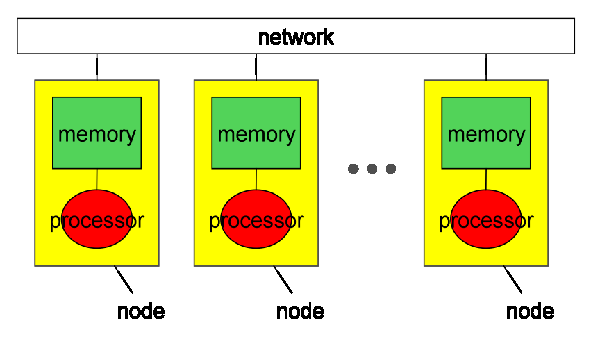
\includegraphics[width=12cm]{figs/Fig1.eps}
  \caption{Hardware Model}\label{fig1}
\end{myfigure}

\section{Execution Model}

The XcalableMP runtime system creates a team of threads on each node
when starting the user program execution. This team of threads is
composed by a single master thread and serveral additional worker
threads.

An XcalableMP program execution is based on the Single Program
Multiple Data (SPMD) model, where the master thread on each node
starts execution from the same main routine and keeps executing the
same code independently (i.e. asynchronously), as if an implicit
tasklet region encloses the whole program, until it encounters an
XcalableMP construct.

The set of nodes on each of which a thread executes a procedure, a
statement, a loop, a block, etc. is referred to as its executing node
set and determined by the innermost task, loop, or array directive
surrounding it dynamically, or at runtime.

The current (executing) node set is the executing node set for the
current context, which is managed by the XcalableMP runtime system on
each node. The current node set at the beginning of the
program execution, or the entire node set, is a node set that contains
all the available nodes, which can be specified in an
implementation-dependent way (e.g. through a command-line option).

When a thread encounters at runtime either a loop, array, or task
construct, and is executed on a node in the node set specified by
the on clause of the directive, it updates the current node set with
the specified one and executes the body of the construct, after which
it resumes the last executing node set and proceeds to execute the
following statements.

Particularly when a thread encounters a loop or an array construct, it
executes the loop body or the array assignment in parallel with
threads on other nodes, so that each iteration of the loop or each
element of the assignment is independently executed on the node where
the specified data element resides.

When a thread encounters a synchronization or a communication
directive, synchronization or communication might occur between it and
threads on other nodes. That is, such global constructs should be
performed collectively on the current nodes. Note that neither
synchronizations nor communications occur without these constructs
specified.

When a thread encounters a tasklet or a taskletloop construct, a new
tasklet is generated on the node. Execution of explicitly generated
tasklets is assigned to one of the threads on the node, subject to the
thread’s availability to execute work. Thus, execution of the new
tasklet could be immediate, or deferred until later according to the
tasklet scheduling constraint and thread availability.

The tasklet scheduling constraint is as follows:

\begin{itemize}
  \item A dependent tasklet shall not be scheduled until its task
		dependences are fulfilled.
\end{itemize}

%%%

% An {\XMP} program execution is based on the Single Program Multiple Data
% (SPMD) model, where each node starts execution from the same main
% routine and keeps executing the same code independently
% (i.e. asynchronously), which is referred to as the {\it \Term{replicated
% execution}}, until it encounters an {\XMP} construct.

% A set of nodes that executes a procedure, a statement, a loop,
% a block, etc. is referred to as its {\it \Term{executing node set}} and
% determined by the innermost {\tt task}, {\tt loop} or {\tt array}
% directive surrounding it dynamically, or at runtime.
% %
% The {\it \Term{current executing node set}} is an executing node set of
% the current context, which is managed by the {\XMP} runtime system on
% each node.

% The current executing node set at the beginning of the program
% execution, or {\it \Term{primary node set}}, is a node set that
% contains all the available nodes, which can be specified in an 
% implementation-dependent way (e.g. through a command-line option).

% When a node encounters at runtime either a {\tt loop}, {\tt array}, or
% {\tt task} construct, and is contained by the node set specified by the
% {\tt on} clause of the directive, it updates the current executing node
% set with the specified one and executes the body of the construct, after
% which it resumes the last executing node set and proceeds to execute the
% following statements.

% Particularly when a node in the current executing node set encounters a
% {\tt loop} or an {\tt array} construct, it executes the loop or the array
% assignment in parallel with other nodes, so that each iteration of the
% loop or element of the assignment is independently executed by the node
% where a specified data element resides.

% When a node encounters a synchronization or a communication directive,
% synchronization or communication occurs between it and other nodes.
% %
% That is, such {\it \Term{global constructs}} are performed collectively
% by the current executing nodes.
% %
% Note that neither synchronizations nor communications occur without these
% constructs specified.

\section{Base Languages}

The XcalableMP language specification is defined on Fortran, C, and C++
as base languages. More specifically, the base language of XcalableMP
Fortran is Fortran 2008, that of XcalableMP C ISO is C99, and that of
XcalableMP C++ is C++11.
